\textit{Analógimôn Go} é um jogo bastante popular. Em sua jornada, o jogador percorre diversas
cidades capturando pequenos monstrinhos virtuais, chamados \textit{analógimôns}.
Você acabou de chegar em uma cidade que contém o último analógimôn que falta
para sua coleção!

A cidade pode ser descrita como um \textit{grid} de $N$ linhas e $M$ colunas.
Você está em uma dada posição da cidade, enquanto o último analógimôn está em
outra posição da mesma cidade. A cada segundo, você pode se mover (exatamente) uma
posição ao norte, ao sul, a leste ou a oeste. Considerando que o analógimôn não
se move, sua tarefa é determinar o menor tempo necessário para
ir até a posição do monstrinho.
A figura descreve o exemplo da
entrada, e apresenta um caminho percorrido em 5 segundos. Outros caminhos
percorridos no mesmo tempo são possíveis, mas não há outro caminho que pode ser
percorrido em um tempo menor.

\begin{center}
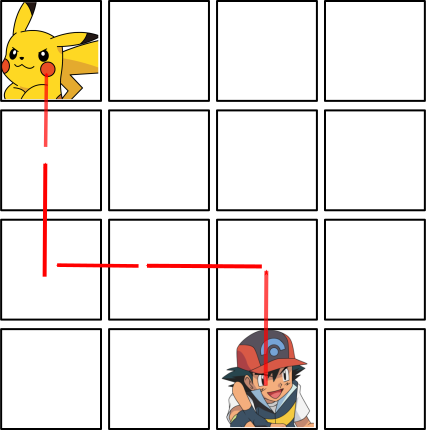
\includegraphics[scale=0.4]{ultimo/ultimo.pdf}
\end{center}

\subsection*{Entrada}

A primeira linha contém dois inteiros $N$ e $M$ ($2 \leq N, M \leq 100$), o
número de linhas e de colunas na cidade, respectivamente. As próximas $N$ linhas
contém $M$ inteiros cada, descrevendo a cidade. O inteiro $0$ indica uma posição
em branco; o inteiro $1$ indica a sua posição na cidade; o inteiro $2$ indica a
posição do analógimôn na cidade.
É garantido que haverá exatamente um inteiro
$1$ e exatamente um inteiro $2$ na descrição da cidade, e que os demais inteiros
serão iguais a $0$.

\subsection*{Saída}

Imprima uma linha contendo o menor tempo necessário para ir até o
monstrinho, em segundos.

\begin{table}[!h]
\centering
\begin{tabular}{|l|l|}
\hline
\begin{minipage}[t]{3in}
\textbf{Exemplo de entrada}
\begin{verbatim}
4 4
2 0 0 0
0 0 0 0
0 0 0 0
0 0 1 0
\end{verbatim}
\vspace{1mm}
\end{minipage}
&

\begin{minipage}[t]{3in}
\textbf{Exemplo de saída}
\begin{verbatim}
5
\end{verbatim}
\vspace{1mm}
\end{minipage} \\
\hline
\end{tabular}
\end{table}
